% для компиляции в lualatex!!
\documentclass[12pt, a4paper]{article}
\usepackage[english,russian]{babel}
\usepackage[warn]{mathtext}
%\usepackage[T2A]{fontenc}
%\usepackage[utf8]{inputenc}

\usepackage{xecyr} % Продукт Вашего покорного слуги ;)

\setmainfont{DejaVu Serif}

\usepackage{color}
\usepackage{amssymb,amsmath}
\usepackage{graphicx}
\usepackage{multicol}

\textheight=24cm           % высота текста
\textwidth=16cm            % ширина текста
\oddsidemargin=0pt         % отступ от левого края
\topmargin=-1.5cm          % отступ от верхнего края
\parindent=24pt            % абзацный отступ
\parskip=0pt               % интервал между абзацами
\tolerance=2000            % терпимость к "жидким" строкам
\flushbottom               % выравнивание высоты страниц
%\def\baselinestretch{1.5} % печать с большим интервалом

%\title{}
%\author{\copyright~~С.А.~Назарова \thanks{e-mail:~sophia.nazarova@gmail.com}}
%\date{}


\begin{document}

\section{Динамика обилия {\it M.~balthica}.}
\subsection{Эстуарий р.~Лувеньги.}

На литорали в эстуарии реки Лувеньги средняя плотность поселений маком за период с $1992$ по $2012$ год колебалась от $55~(26,8)$ в $1992$ до $9200~(39,8)$~экз./м$^2$ в $1998$ году (рис. \ref{ris:dynamic_Kandalaksha_all}). 
При этом столь высокая численность в 1998 году была связана с особями длиной менее $1$~мм (рис. \ref{ris:dynamic_Kandalaksha_all2}) --- численность моллюсков крупнее $1$~мм составляла всего $750~(2,03)$~экз./м$^2$.
Для анализа динамики обилия, на наш взгляд, более информативно рассматривать численность без учета вновь осевших особей. 
\textcolor{red}{ОБЪЯСНЯТЬ ПРО ПОПОЛНЕНИЕ ПОСЕЛЕНИЯ ТУТ ИЛИ ГДЕ?}. 
Поскольку материал собирали в конце июля --- начале августа, то мы считаем спатом всех особей длиной менее $1$~мм. \textcolor{red}{сюда бы ссылку на размер спата в белом? Зубаха, Полоскин, Гольцев?} 
В этом случае можно говорить о двух периодах, различающихся по численности: с $1992$ по $1998$ год --- период относительно низкой численности (средняя численность за весь период $340~(15,4)$~экз./м$^2$), и с $1999$ по $2012$ год --- относительно высокой ($2000~(5,4)$~экз./м$^2$) (достоверные различия по критерию Манна-Уитни $W = 6, p-value = 4.528e-13$).
Во второй период минимальная плотность поселения была отмечена в 2006 году и сставляла $993~(13,2)$~экз./м$^2$). 
Периоды с 1999 по 2006 и с 2007 по 2012 годы не различаются по численности (критерий Манна-Уитни $W = 432, p-value = 0.2132$).


\subsection{Литораль Западной Ряшковой салмы о.~Ряшкова.}
На данном участке литорали средняя плотность поселений {\it M.~balthica} за период с $1994$ по $2012$ год колебалась от $220~(40,9)$~экз./м$^2$ до $9285~(16,4)$~экз./м$^2$ (рис. \ref{ris:dynamic_Kandalaksha_all}).




\newpage
\begin{figure}[h]

\begin{minipage}[b]{.46\linewidth}
%Фигурка в первом ряду слева размер отведенный под весь этот объект -- 0.46 от ширины строки
%Параметр [b] означает, что выравнивание этих министраниц будет по нижнему краю
\begin{center}
	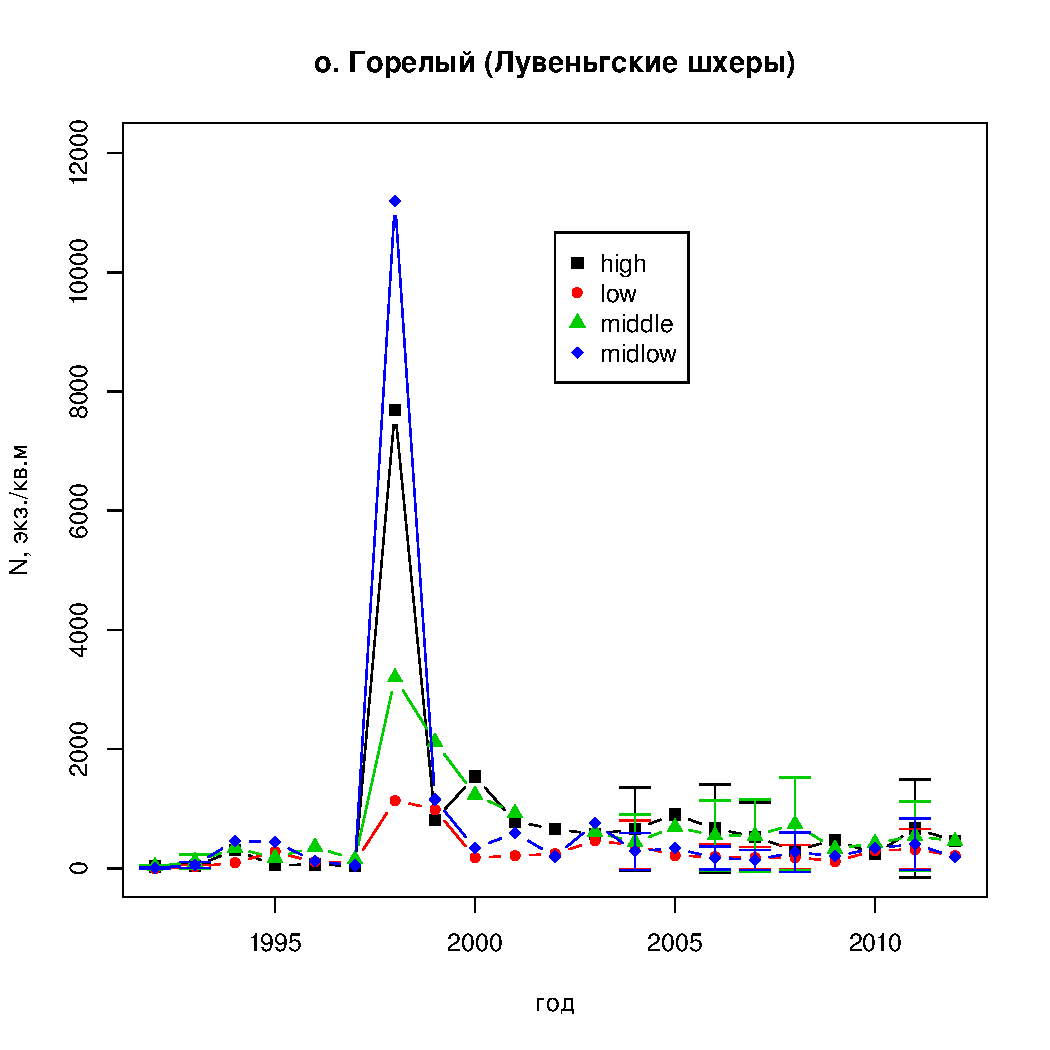
\includegraphics[width=65mm]{../White_Sea/Luvenga_Goreliy/N_dynamic.pdf}
\end{center}
\end{minipage}
%
\hfil %Это пружинка отодвигающая рисунки друг от друга
%
\begin{minipage}[b]{.46\linewidth}
%Следующий рисунок - первый ряд справа %DUNGEON S_4 \ AB
\begin{center}
	\includegraphics[width=65mm]{../White_Sea//Luvenga_II_razrez/N_dynamic.pdf}
\end{center}
\end{minipage}


%\smallskip


\begin{minipage}[b]{.46\linewidth}
%Фигурка в первом ряду слева размер отведенный под весь этот объект -- 0.46 от ширины строки
%Параметр [b] означает, что выравнивание этих министраниц будет по нижнему краю
\begin{center}
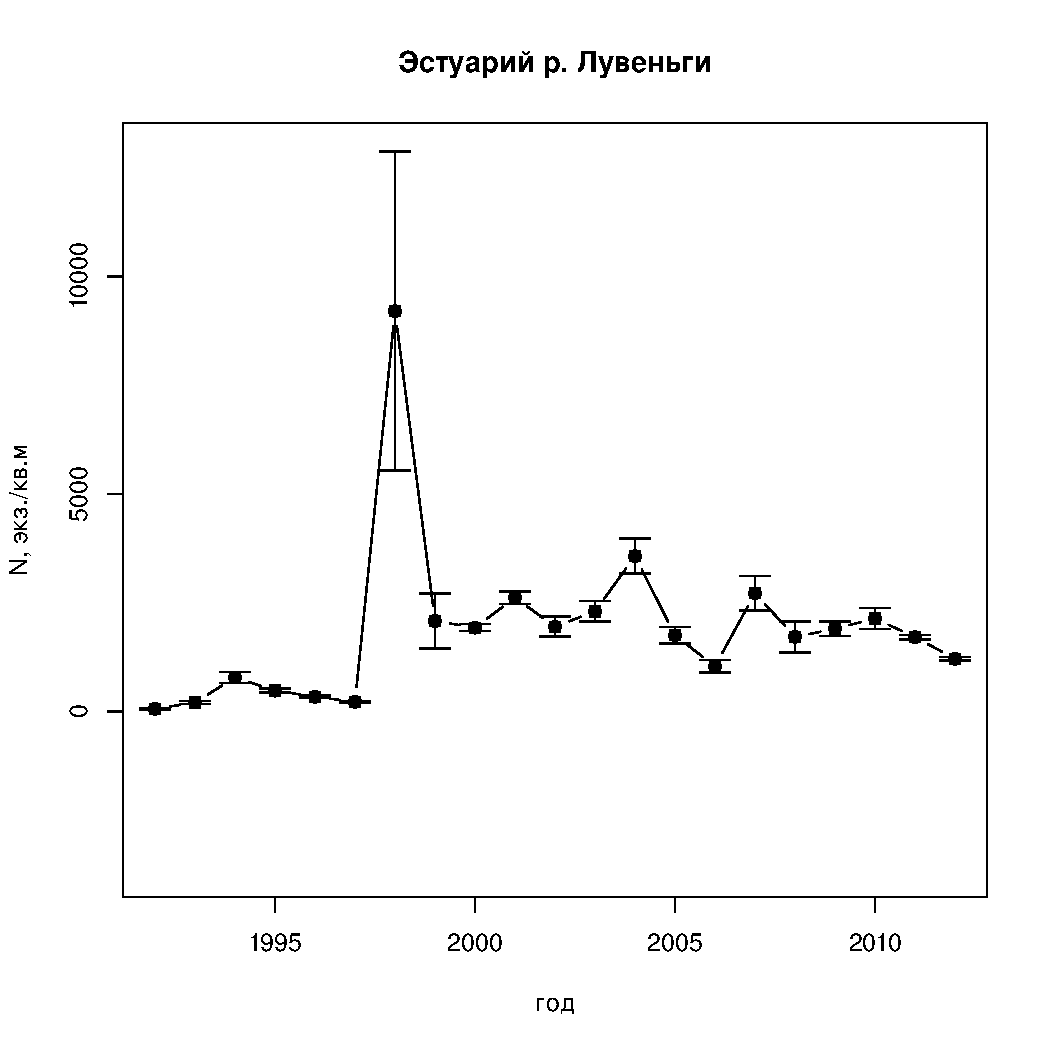
\includegraphics[width=65mm]{../White_Sea/Estuatiy_Luvenga/N_dynamic.pdf}
\end{center}
\end{minipage}
%
\hfil %Это пружинка отодвигающая рисунки друг от друга
%
\begin{minipage}[b]{.46\linewidth}
%Следующий рисунок - первый ряд справа %DUNGEON S_4 \ AB
\begin{center}
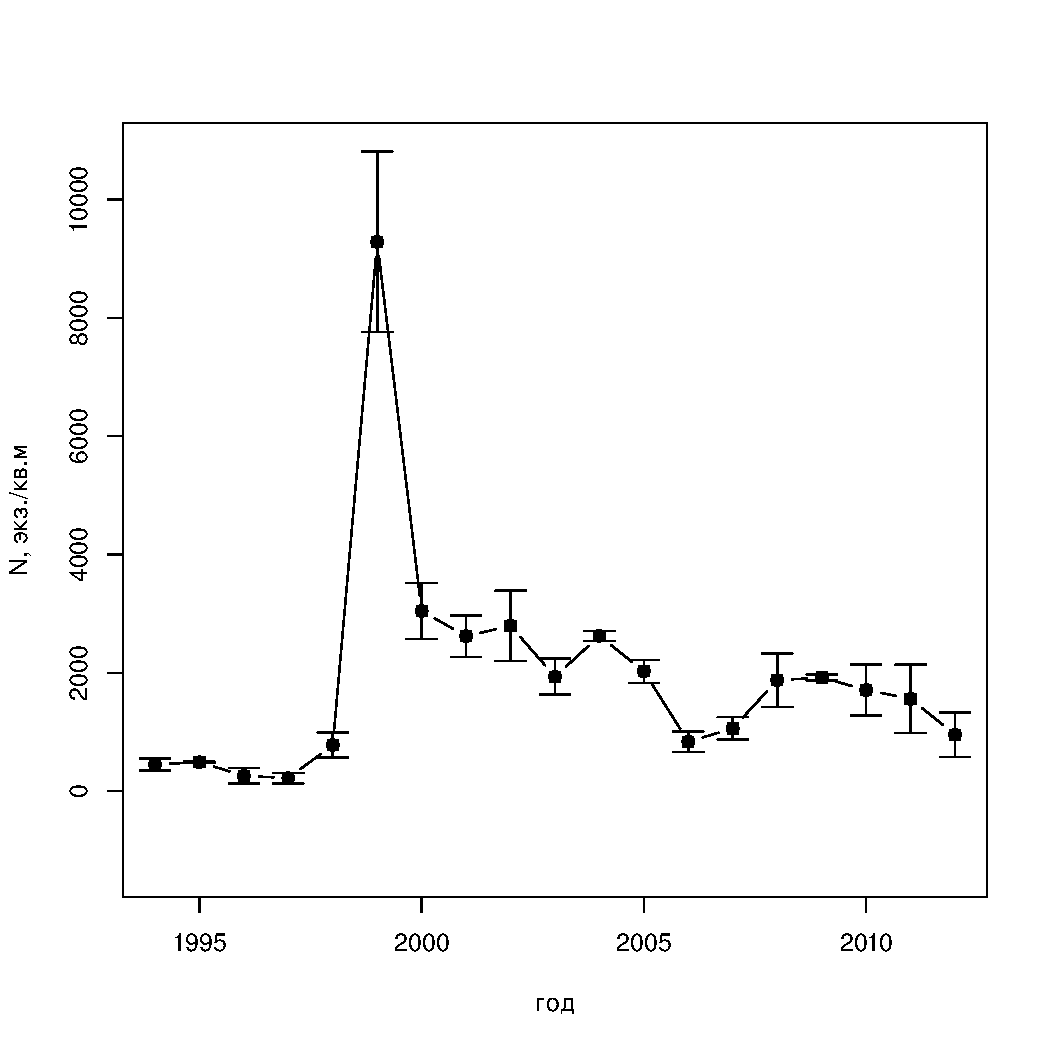
\includegraphics[width=65mm]{../White_Sea/Ryashkov_ZRS/N_dynamic.pdf}
\end{center}
\end{minipage}

%\smallskip

\begin{minipage}[b]{.46\linewidth}
%Фигурка в первом ряду слева размер отведенный под весь этот объект -- 0.46 от ширины строки
%Параметр [b] означает, что выравнивание этих министраниц будет по нижнему краю
\begin{center}
\includegraphics[width=65mm]{../White_Sea/Ryashkov_YuG/N_dynamic.pdf}
\end{center}
\end{minipage}
%
\hfil %Это пружинка отодвигающая рисунки друг от друга
%
\begin{minipage}[b]{.46\linewidth}
%Следующий рисунок - первый ряд справа %DUNGEON S_4 \ AB
\begin{center}
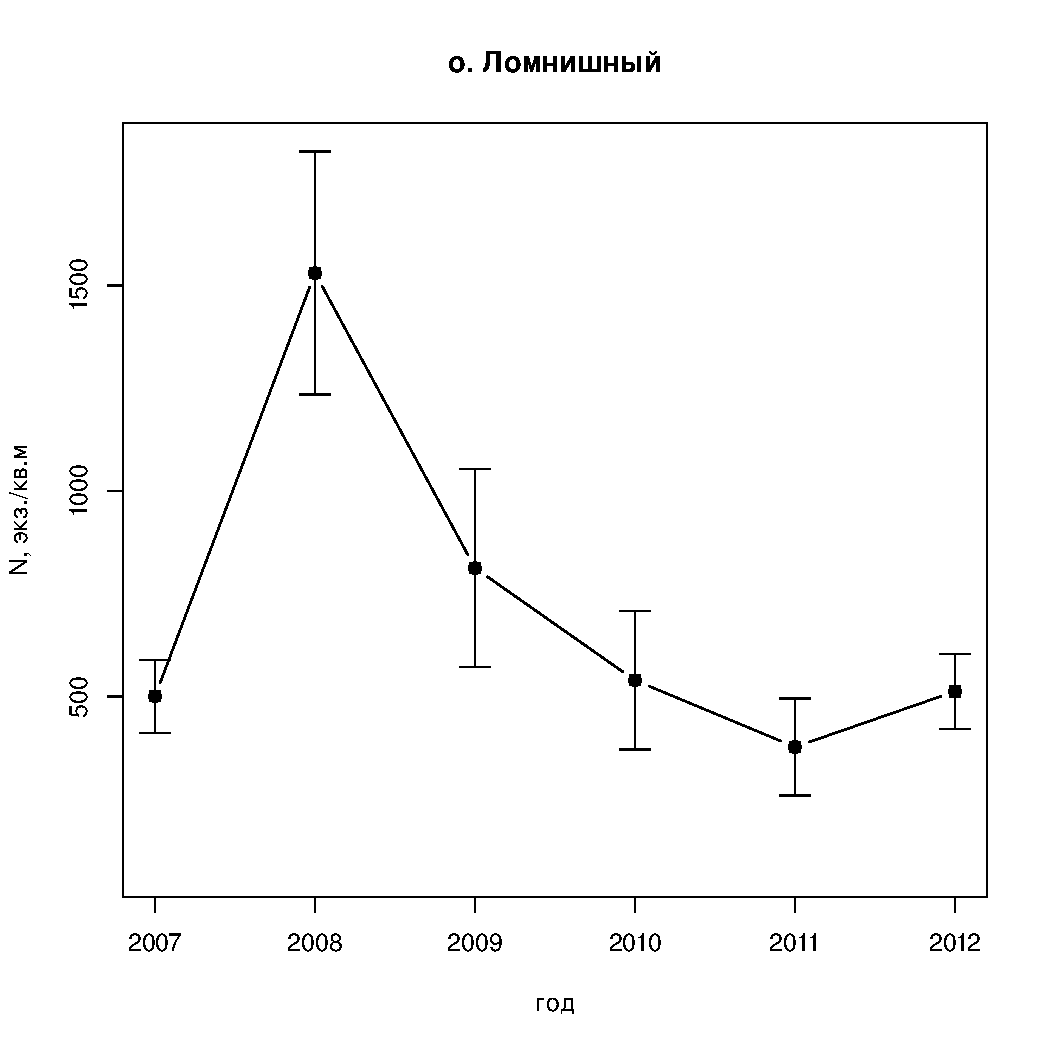
\includegraphics[width=65mm]{../White_Sea/Lomnishniy/N_dynamic.pdf}
\end{center}
\end{minipage}

%\smallskip


\caption{Динамика плотности поселений {\it Macoma balthica} в вершине Кандалакшского залива}
\label{ris:dynamic_Kandalaksha_all}
\end{figure}

\newpage
\begin{figure}[h]

\begin{minipage}[b]{.46\linewidth}
%Фигурка в первом ряду слева размер отведенный под весь этот объект -- 0.46 от ширины строки
%Параметр [b] означает, что выравнивание этих министраниц будет по нижнему краю
\begin{center}
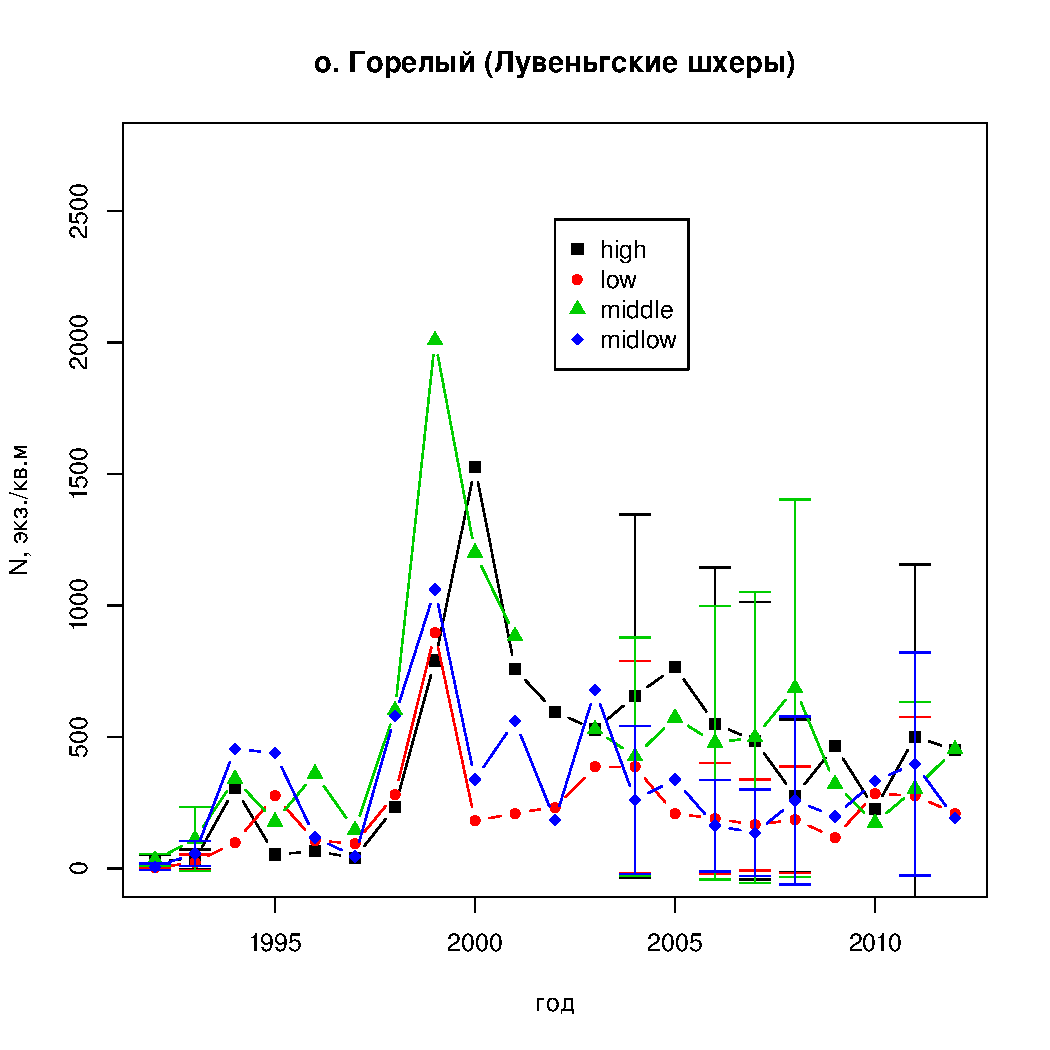
\includegraphics[width=65mm]{../White_Sea/Luvenga_Goreliy/N2_dynamic.pdf}
\end{center}
\end{minipage}
%
\hfil %Это пружинка отодвигающая рисунки друг от друга
%
\begin{minipage}[b]{.46\linewidth}
%Следующий рисунок - первый ряд справа %DUNGEON S_4 \ AB
\begin{center}
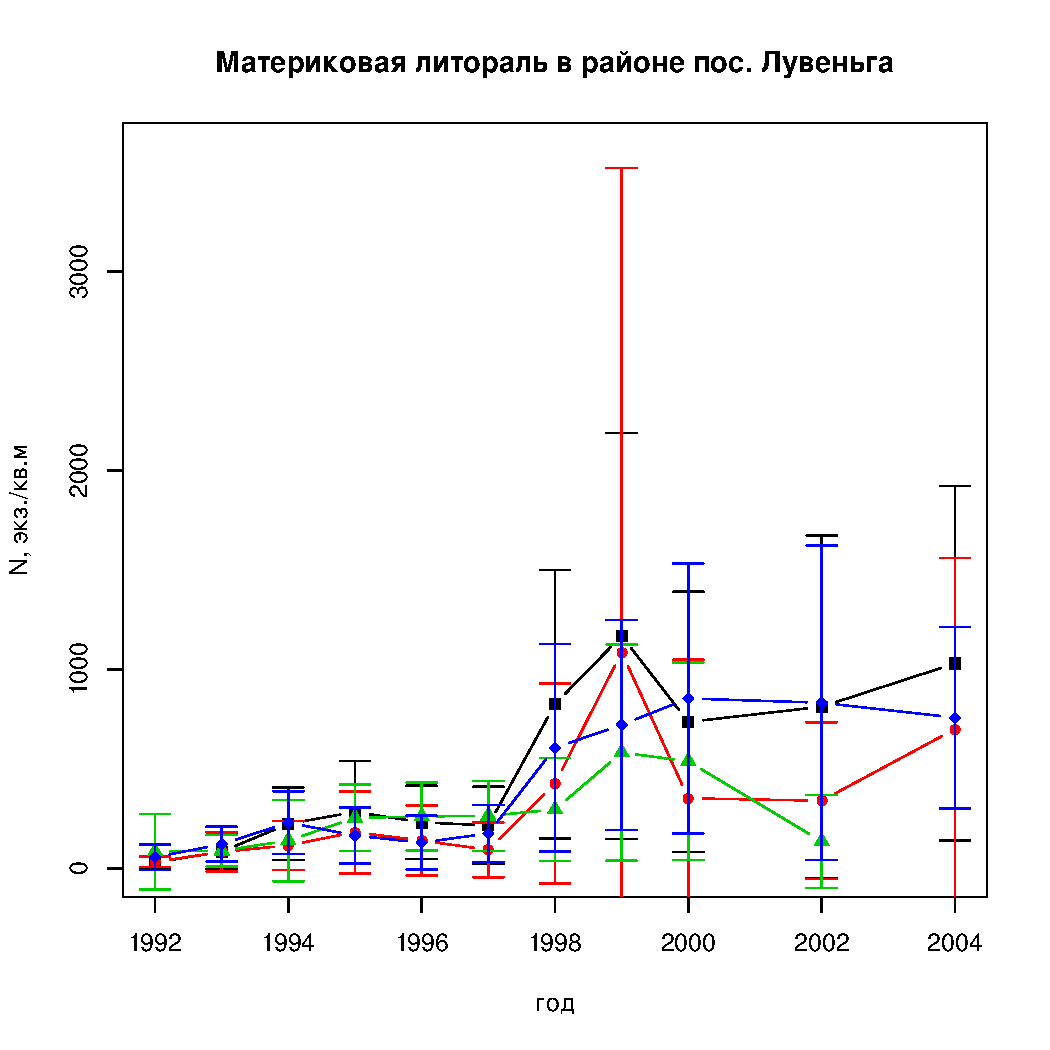
\includegraphics[width=65mm]{../White_Sea//Luvenga_II_razrez/N2_dynamic.pdf}
\end{center}
\end{minipage}

%\smallskip


\begin{minipage}[b]{.46\linewidth}
%Фигурка в первом ряду слева размер отведенный под весь этот объект -- 0.46 от ширины строки
%Параметр [b] означает, что выравнивание этих министраниц будет по нижнему краю
\begin{center}
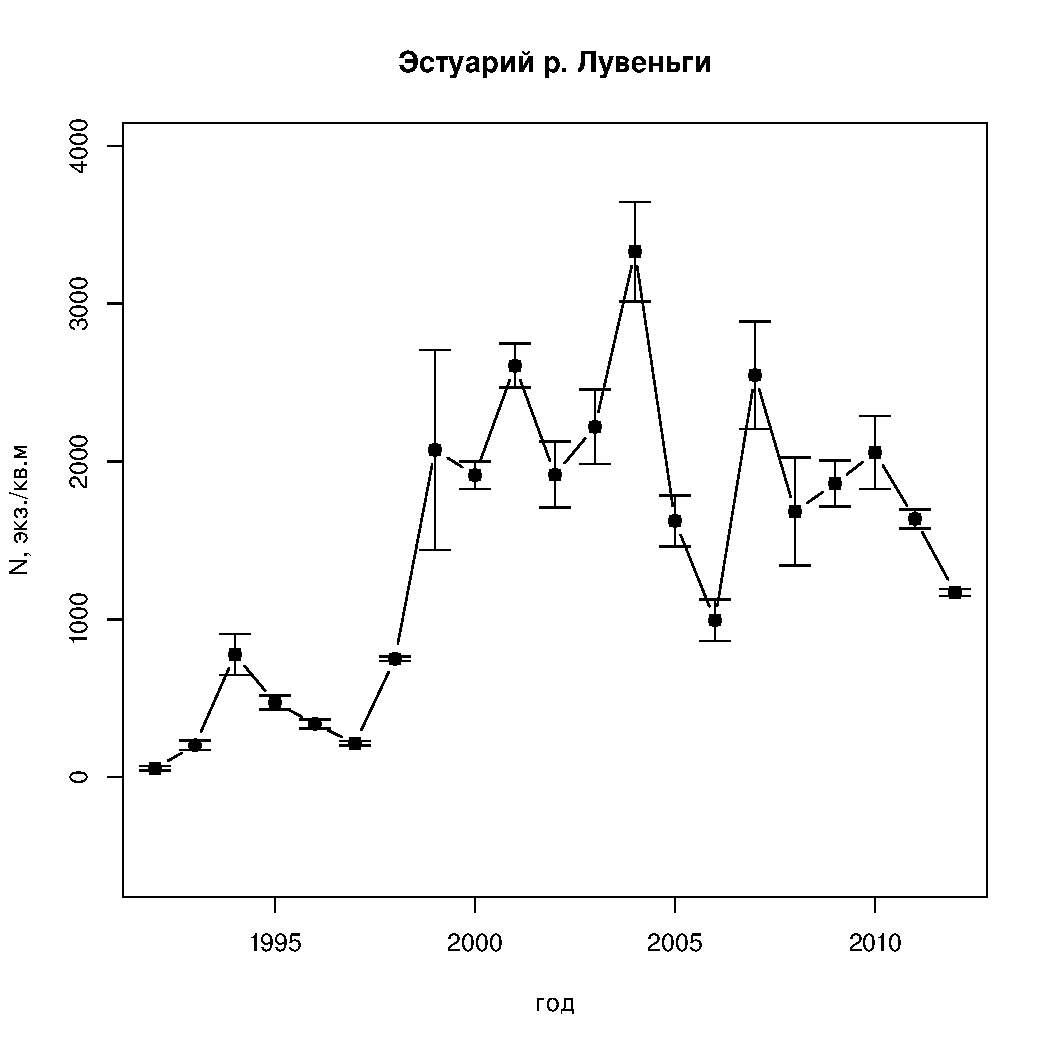
\includegraphics[width=65mm]{../White_Sea/Estuatiy_Luvenga/N2_dynamic.pdf}
\end{center}
\end{minipage}
%
\hfil %Это пружинка отодвигающая рисунки друг от друга
%
\begin{minipage}[b]{.46\linewidth}
%Следующий рисунок - первый ряд справа %DUNGEON S_4 \ AB
\begin{center}
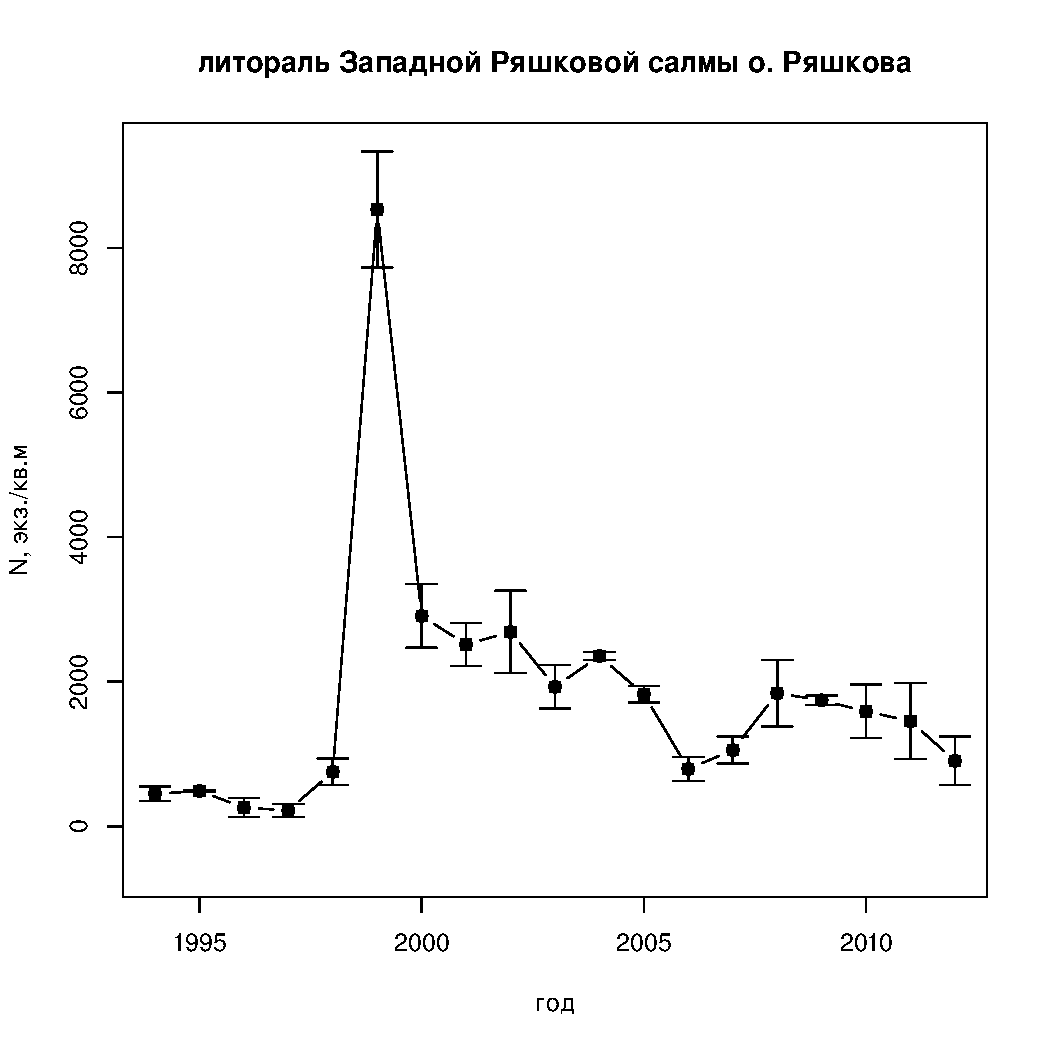
\includegraphics[width=65mm]{../White_Sea/Ryashkov_ZRS/N2_dynamic.pdf}
\end{center}
\end{minipage}

%\smallskip

\begin{minipage}[b]{.46\linewidth}
%Фигурка в первом ряду слева размер отведенный под весь этот объект -- 0.46 от ширины строки
%Параметр [b] означает, что выравнивание этих министраниц будет по нижнему краю
\begin{center}
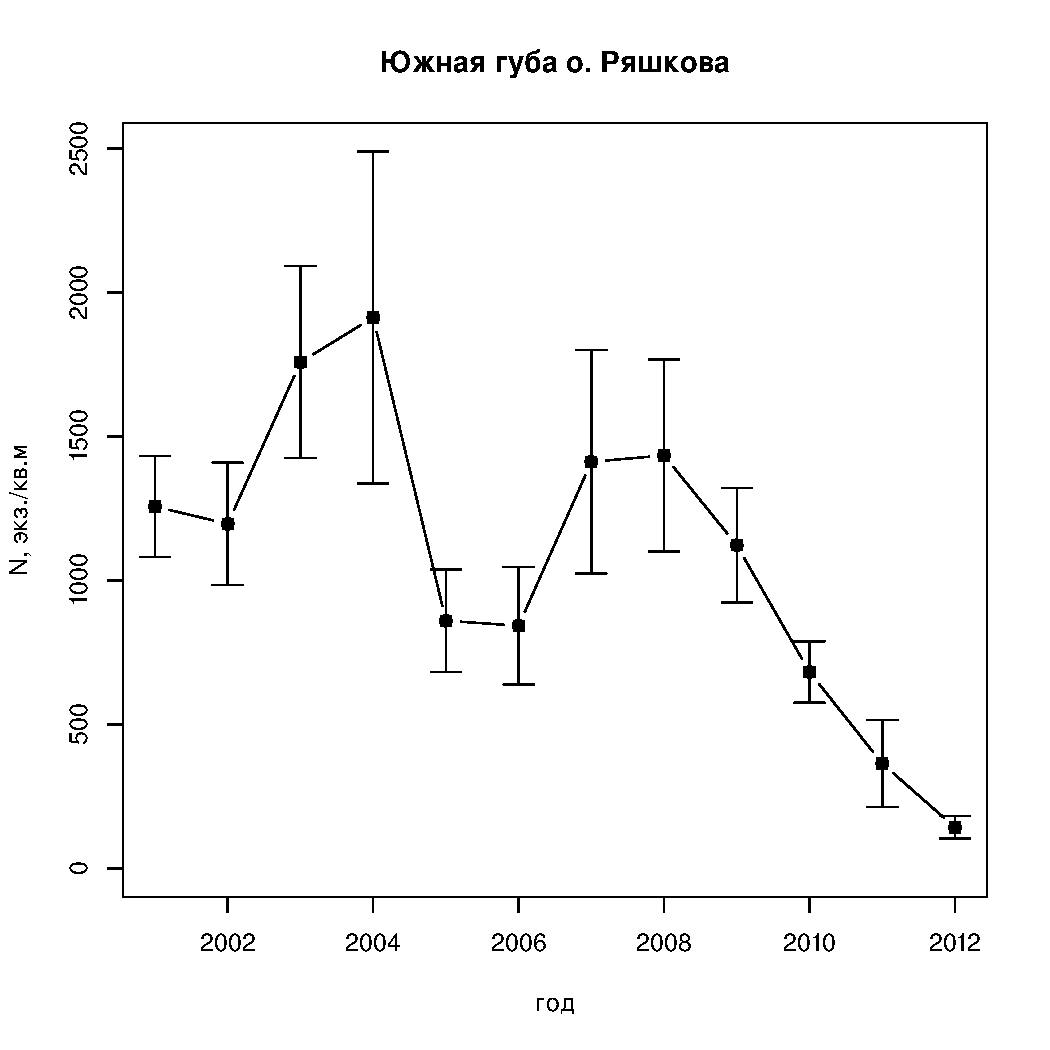
\includegraphics[width=65mm]{../White_Sea/Ryashkov_YuG/N2_dynamic.pdf}
\end{center}
\end{minipage}
%
\hfil %Это пружинка отодвигающая рисунки друг от друга
%
\begin{minipage}[b]{.46\linewidth}
%Следующий рисунок - первый ряд справа %DUNGEON S_4 \ AB
\begin{center}
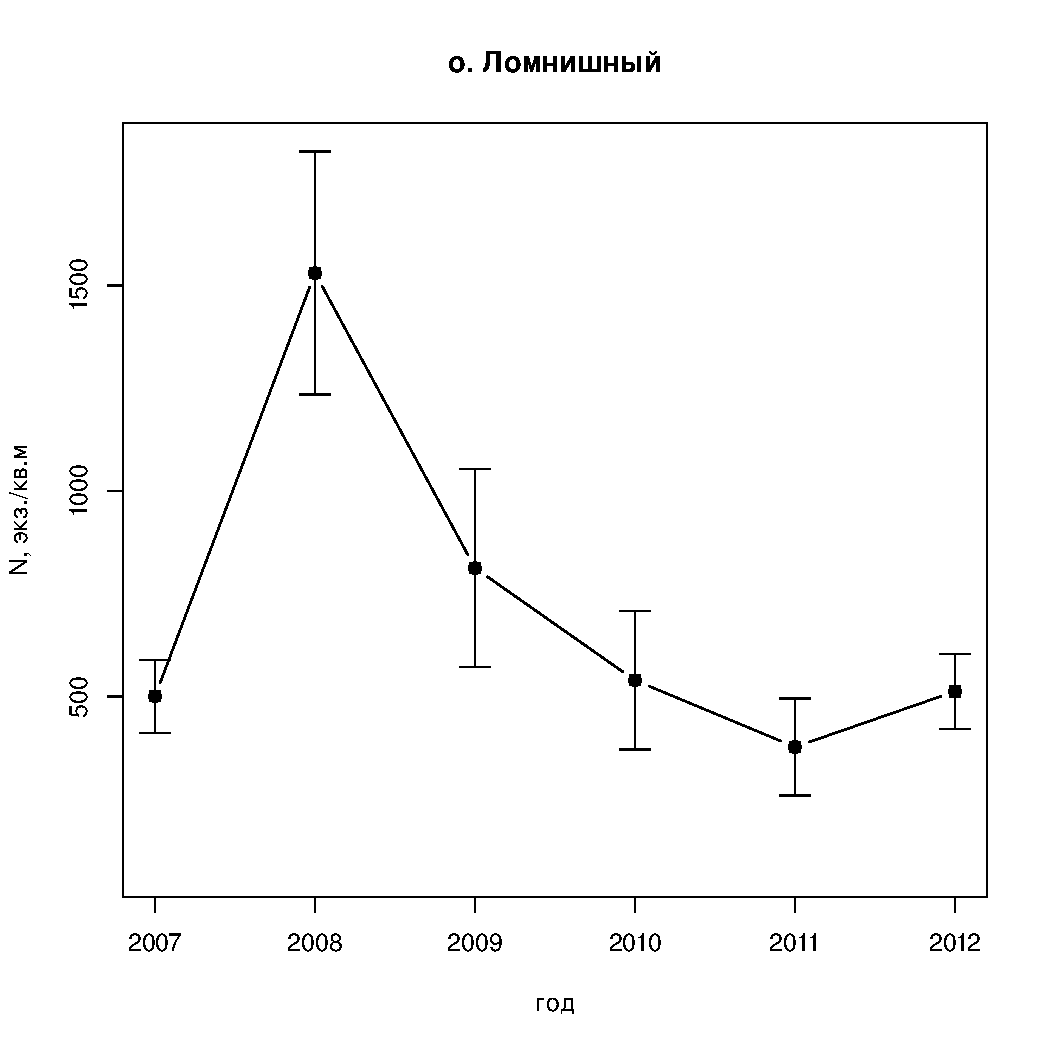
\includegraphics[width=65mm]{../White_Sea/Lomnishniy/N2_dynamic.pdf}
\end{center}
\end{minipage}

%\smallskip


\caption{Динамика численности {\it Macoma balthica} с длиной раковины более $1$~мм в поселениях вершины Кандалакшского залива}
\label{ris:dynamic_Kandalaksha_all2}
\end{figure}

\end{document}
